% !TeX spellcheck = it_IT
% !TXS template
\documentclass[italian]{article}
\usepackage[T1]{fontenc}
\usepackage[utf8]{inputenc}
\usepackage{lmodern}
\usepackage[a4paper,top=3cm,bottom=3cm,left=2.5cm,right=2.5cm]{geometry}
\usepackage[italian]{babel}
\usepackage{enumitem}
\usepackage[fleqn]{amsmath}
\usepackage{amssymb}
\usepackage{mathtools}% http://ctan.org/pkg/mathtools
\usepackage{cancel}
\usepackage{color}
\usepackage[usenames,dvipsnames]{xcolor}
\usepackage{units}
\usepackage{hyperref}
\usepackage{textcomp}
\usepackage{soul}
\usepackage{listings}
\usepackage{pifont} %https://www.rpi.edu/dept/arc/training/latex/LaTeX_symbols.pdf
\usepackage{fontspec}
\usepackage{fontawesome}
\usepackage{mdframed}
\usepackage{pgf,tikz}
\usepackage{mathrsfs}
\usetikzlibrary{arrows}
\usepackage{multicol}
\usepackage{titlesec}

\hypersetup{
	colorlinks,
	citecolor=black,
	filecolor=black,
	linkcolor=black,
	urlcolor=blue
}

% SubSubSubSection
%\titleclass{\subsubsubsection}{straight}[\subsection]
%\newcounter{subsubsubsection}[subsubsection]
%\renewcommand\thesubsubsubsection{\thesubsubsection.\arabic{subsubsubsection}}
%\renewcommand\theparagraph{\thesubsubsubsection.\arabic{paragraph}} % optional; useful if paragraphs are to be numbered
%\titleformat{\subsubsubsection}
%{\normalfont\normalsize\bfseries}{\thesubsubsubsection}{1em}{}
%\titlespacing*{\subsubsubsection}
%{0pt}{3.25ex plus 1ex minus .2ex}{1.5ex plus .2ex}

%\makeatletter
%\renewcommand\paragraph{\@startsection{paragraph}{5}{\z@}%
%	{3.25ex \@plus1ex \@minus.2ex}%
%	{-1em}%
%	{\normalfont\normalsize\bfseries}}
%\renewcommand\subparagraph{\@startsection{subparagraph}{6}{\parindent}%
%	{3.25ex \@plus1ex \@minus .2ex}%
%	{-1em}%
%	{\normalfont\normalsize\bfseries}}
%\def\toclevel@subsubsubsection{4}
%\def\toclevel@paragraph{5}
%\def\toclevel@paragraph{6}
%\def\l@subsubsubsection{\@dottedtocline{4}{7em}{4em}}
%\def\l@paragraph{\@dottedtocline{5}{10em}{5em}}
%\def\l@subparagraph{\@dottedtocline{6}{14em}{6em}}
%\makeatother
%\setcounter{secnumdepth}{4}
%\setcounter{tocdepth}{4}
% End SubSubSubSection

\renewcommand{\labelitemii}{$\circ$}
\newcommand{\powerset}[1]{\mathcal{P}(#1)}

\newcommand\x{\times}
\newcommand{\linea}{\begin{center}\rule{5cm}{1pt}\end{center}}
\newcommand{\crossmark}{\textcolor{red}{\text{\ding{56}}}}
\renewcommand{\checkmark}{\textcolor{ForestGreen}{\text{\ding{52}}}}
\newcommand{\ins}[1]{\text{$\mathbb{#1}$}}
\newcommand{\dateright}[1]{\normalfont{\normalsize{\hfill #1 \\}}}
\renewcommand{\dim}[1]{\text{dim$\left(#1\right)$}}
\newcommand{\taleche}{\;|\;}


\let\oldexists\exists
\renewcommand{\exists}{\text{$\;\oldexists$}}

\newcommand{\exercize}{\text{\faPencil $\;$ Esercizio }}
\newcommand{\homeExercize}{\text{\faHome $\;$ Esercizio per casa}}
\newcommand{\example}{\text{\faCircleArrowRight $\;$ Esempio }}


\definecolor{ao(english)}{rgb}{0.0, 0.5, 0.0}

\lstset{language=C,
	basicstyle=\ttfamily,
	keywordstyle=\color{blue}\ttfamily,
	stringstyle=\color{red}\ttfamily,
	commentstyle=\color{ao(english)}\ttfamily,
	morecomment=[l][\color{magenta}]{\#}
}

\author{Giacomo De Liberali}

\begin{document}
	
\title{Calcolabilità e Linguaggi Formali}
\maketitle

\tableofcontents
\pagebreak

\section{Introduzione}
\dateright{21 Settembre 2017}
Gli argomenti trattati in questo corso sono:

\begin{enumerate}
	\item Teoria degli automi (capitoli $1,2,3$)
	\item Calcolabilità: cosa si può computare? (capitili $3,4,5$) 
	\item Complessità delle soluzioni
\end{enumerate}

\section{Linguaggi regolari}
Il modello di computazione più elementare sono gli automi a stati finiti. Andiamo a rappresentare tramite un automa una porta con una bilancia da ogni lato che permetta l'accesso alle persone e impedisca alla porta stessa di colpire qualcuno:

\begin{center}
	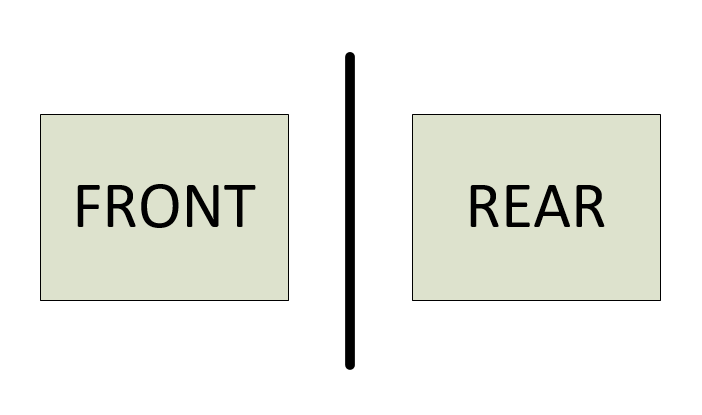
\includegraphics[width=0.3\linewidth]{images/door}
\end{center}
La pressione della pedana \textit{Font} comporterà quindi l'apertura della porta. I possibili input sono quattro:
\begin{enumerate}
	\item Front
	\item Rear
	\item Both
	\item Neither
\end{enumerate}

e rappresentati in un automa:

\begin{center}
	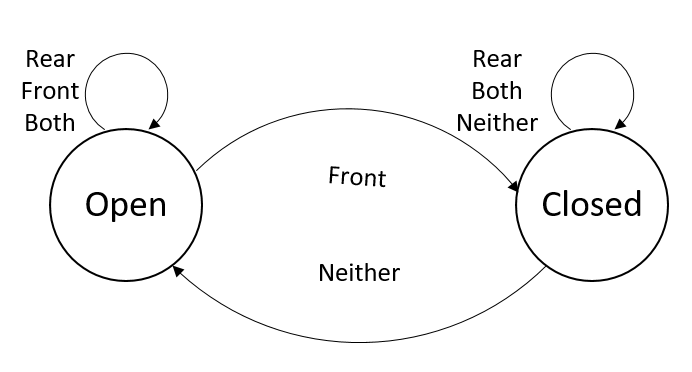
\includegraphics[width=0.5\linewidth]{images/automa1}
\end{center}

\pagebreak

\section{Automa a stati finiti}
\subsection{Definizione}
\label{sec:automDefinition}
Un automa a stati finiti è una 5-tupla $(Q,\;\Sigma,\;\delta,\;q_0,\;F)$ dove:
\begin{enumerate}
	\item $Q$ è un insieme finito di stati
	\item $\Sigma$ è un insieme finito di simboli (detto \textit{alfabeto})
	\item $\delta$ è la \textit{funzione di transizione} che data una coppia stato-alfabeto ritorna uno stato: $\delta: Q\times\Sigma \to Q$
	\item $q_0 \in Q$ è lo stato iniziale (negli automi è ammesso solo \underline{uno} stato iniziale)
	\item $F \subseteq Q$ è un insieme degli stati finali (o \textit{accettanti})
\end{enumerate}
\example
\begin{center}
	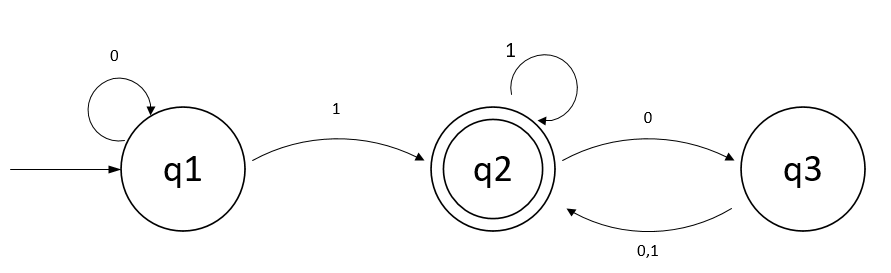
\includegraphics[width=0.8\linewidth]{images/automa2}
\end{center}
L'automa può essere rappresentato formalmente mediante la seguente sintassi:
\[
	A = (\{q_1,q_2,q_3\},\; \{0,1\},\; \delta,\; q_1,\; \{q_2\}) 
\]
dove $\delta$ è definita come:
\begin{gather*}
	\delta(q_1,0) = q_1 \qquad \delta(q_1,1) = q_2 \\
	\delta(q_2,0) = q_3 \qquad \delta(q_2,1) = q_2 \\
	\delta(q_3,0) = q_2 \qquad \delta(q_3,1) = q_2
\end{gather*}
Analizzando le stringhe che l'automa accetta, possiamo notare che quelle valide (e quindi accettate) sono tutte quelle che
\begin{enumerate}
	\item finiscono con $1$
	\item oppure finiscono con $0$ e hanno un numero pari di $0$ dopo l'ultimo $1$
\end{enumerate}
Ad esempio, la stringa $1101$ è una stringa valida in quanto alla fine dell'input l'automa è nello stato $q_2$ che è l'unico stato finale.
\pagebreak \\
\example
\begin{center}
	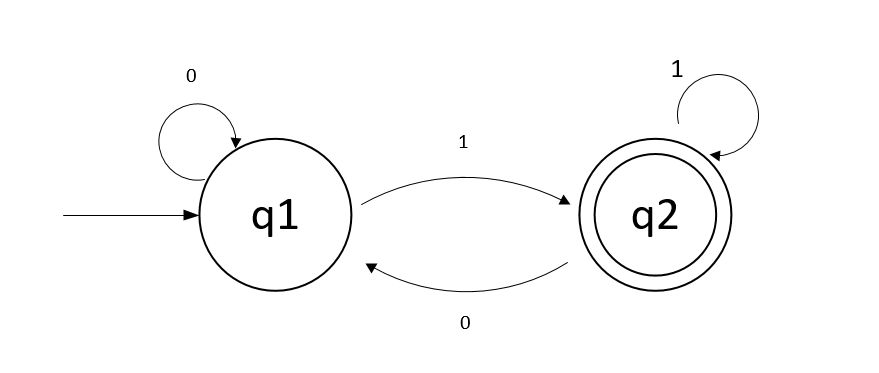
\includegraphics[width=0.5\linewidth]{images/automa3}
\end{center}
Questo automa riconosce stringhe in $\{0,1\}$ che finiscono per $1$. Nel caso di stringa vuota ($\varepsilon$) non entro in nessuno stato e non mi muovo. \\\\
\example
\begin{center}
	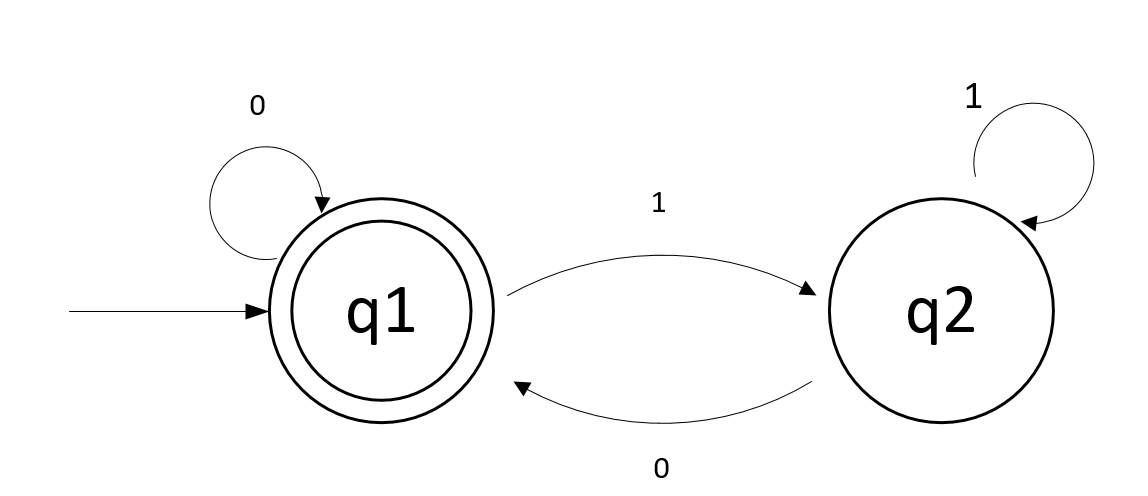
\includegraphics[width=0.5\linewidth]{images/automa4}
\end{center}
Questo automa riconosce stringhe in $\{0,1\}$ che finiscono per $0$ oppure $\varepsilon$.\\\\
\example
\begin{center}
	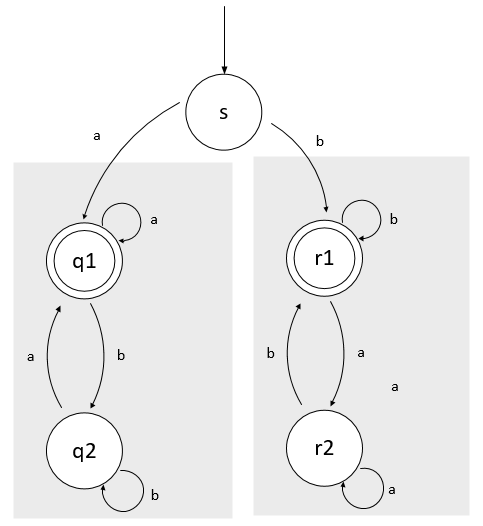
\includegraphics[width=0.5\linewidth]{images/automa5}
\end{center}
Questo automa riconosce stringhe in $\{a,b\}$ che iniziano e finiscono per lo stesso simbolo. In automi come in questo caso è utile poter scomporre il problema in più sotto-problemi Possiamo notare infatti che una volta scelto uno dei due rami che non è possibile passare all'altro. Questo suggerisce di studiare singolarmente i due automi sinistro e destro e infine di comporre la soluzione. \\\\
L'automa di sinistra accetta stringhe che iniziano e finiscono solo per $a$, mentre l'automa di sinistra solo stringhe che iniziano e finiscono per $b$.\\\\
\example
\begin{center}
	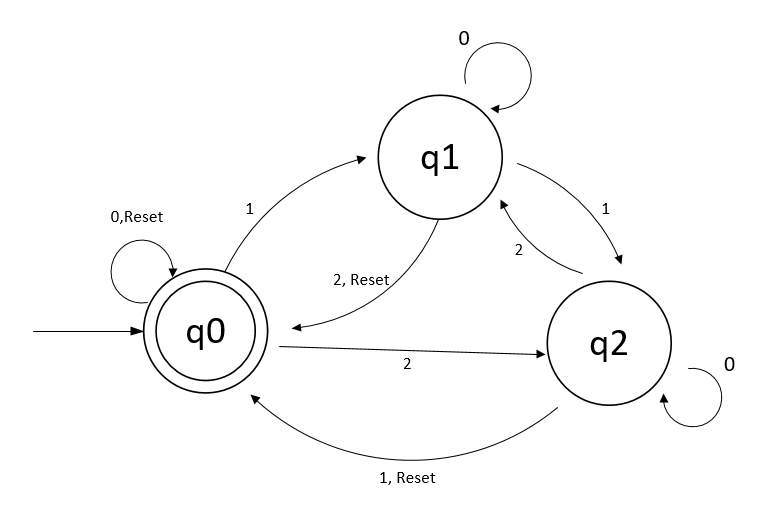
\includegraphics[width=0.5\linewidth]{images/automa6}
\end{center}
Questo automa fa la somma modulo $3$ di tutti i numeri letti in input dopo l'ultimo simbolo di \textit{Reset}, se esiste. 

\subsection{Accettazione di una stringa}
Sia $M = (Q,\;\Sigma,\;\delta,\;q_0,\;F)$ un automa a stati finiti e sia $w = w_1, ..., w_n$ una stringa tale che 
\[
	\forall i \in [1...n] : w_i \in \Sigma
\]
Diciamo che $M$ accetta $w$ se e solo se esiste una sequenza di stati $R_0,R_1,...,R_n \in Q$ tali che
\begin{enumerate}
	\item $R_0 = q_0$ (partendo dal nodo iniziale)
	\item $R_n \in F$ (terminando in uno stato finale)
	\item $\forall i \in [0,n-1] : \sigma(R_i,w_{i+1}) = R_{i+1}$ (per ogni input la \hyperref[sec:automDefinition]{\underline{\textit{funzione di transizione}}} termini in uno stato finale)
\end{enumerate}
$M$ riconosce il linguaggio $A$ se e solo se
\[
	A = \{ w \taleche M \text{ accetta } w \}
\]
Un linguaggio $A$ è \textit{regolare} se e solo se esiste un automa a stati finiti $M$ tale che $M$ riconosce $A$. \\
\pagebreak \\
\example: alfabeto $\{0,1\}$ e vogliamo riconoscere tutte le stringhe con un numero dispari di $1$. L'idea è di avere un bit di informazione, quindi due stati, che mi rappresentano la condizione: ho contanto un numero pari di $1$ oppure ho contanto un numero dispari di $1$. L'automa è il seguente:
\begin{center}
	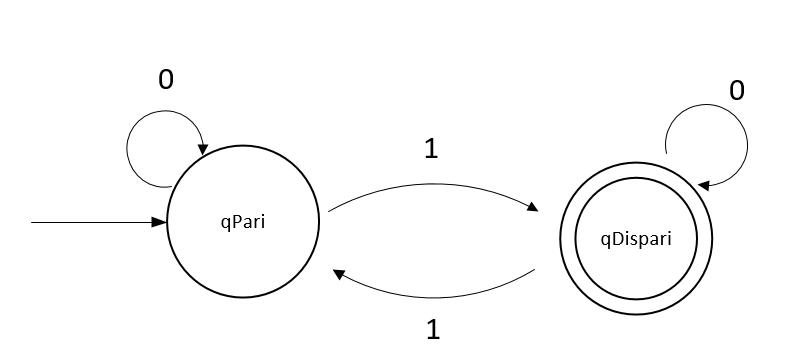
\includegraphics[width=0.5\linewidth]{images/automa7}
\end{center}
\example: alfabeto $\{0,1\}$ e vogliamo riconoscere tutte le stringhe che contengono almeno una volta la sotto-stringa $001$. L'invariante è:
\begin{enumerate}
	\item $q_0$: non ho letto sequenze di $001$
	\item $q_1$: ho letto $0$
	\item $q_2$: ho letto $00$
	\item $q_3$: ho letto $001$
\end{enumerate}
\begin{center}
	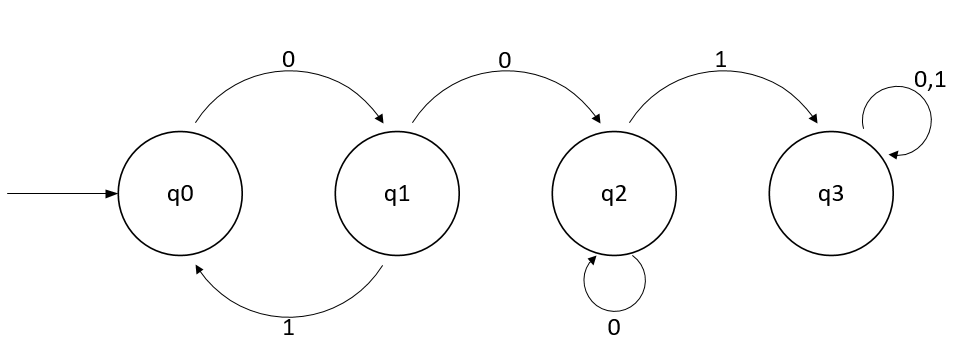
\includegraphics[width=0.6\linewidth]{images/automa8}
\end{center}
\pagebreak
\subsection{Operazioni regolari}
Siano $A$ e $B$ due linguaggi. Definiamo le operazioni regolari \textbf{unione}, \textbf{concatenazione} e \textbf{star} come segue:
\begin{enumerate}
	\item \textbf{Unione}: $A \cup B = \{ x \taleche x \in A  \lor x \in B \}$
	\item \textbf{Concatenazione}: $A \circ B = \{ xy \taleche x \in A  \land y \in B \}$
	\item \textbf{Star}: $A^* = \{ x_1x_2\dots x_n \taleche k \geq 0 \land \forall i \; x_i \in A \}$
\end{enumerate} 
L'operazione \textit{star} è un'operazione unaria e non binaria come le altre due. Si applica quindi ad un solo linguaggio invece che a due. Funziona combinando le stringhe in $A$ con se stesse per ottenere una stringa nel nuovo linguaggio. Poiché ogni numero include $0$ come possibilità, la stringa vuota $\varepsilon$ è sempre un membro di $A^*$, indipendentemente da cosa $A$ sia.\\\\
\example: sia $\Sigma$ l'alfabeto composto dalle $26$ lettere standard $\{ a,b,\dots,z \}$. Se $A = \{ \text{good},\text{bad} \}$ e $B = \{ \text{boy},\text{girl} \}$ allora:
\begin{itemize}[label={}]
	\item $A \cup B = \{ \text{good},\text{bad}, \text{boy},\text{girl} \}$
	\item $A \circ B = \{ \text{goodboy},\text{goodgirl},\text{badboy}, \text{badgirl} \}$
	\item $A^* = \{ \varepsilon, \text{good},\text{bad},\text{goodgood}, \text{goodbad}, \text{badgood}, \\ \text{badbad}, \text{goodgoodgood}, \text{goodgoodbad}, \text{goodbadgood}, \text{goodbadbad}, \dots \}$
\end{itemize}
Una collezione di oggetti si dice chiusa sotto un'operazione se applicando tale operazione ai membri della collezione l'oggetto ritornato è ancora nella collezione di partenza (es. $\mathbb{N}$ è chiuso rispetto al prodotto ma non rispetto alla divisione).

\subsection{Chiusura}
\subsubsection{Rispetto all'unione}
La classe dei linguaggi regolari è chiusa rispetto all'operazione di unione $\cup$.\\\\
Siano $A_1,A_2$ due linguaggi regolari, vogliamo dimostrare che $A_1 \cup A_2$ è un linguaggio regolare. Poiché $A_1$ e $A_2$ sono regolari, sappiamo che esiste un automa a stati finiti $M_1$ che riconosce $A_1$ ed un automa $M_2$ che riconosce $A_2$. Per dimostrare che $A_1 \cup A_2$ è regolare dimostriamo un automa a stati finiti $M$ che riconosce $A_1 \cup A_2$. \\\\
Sia $M_1 = (Q_1,\Sigma,\delta_1,q_1,F_1)$ e sia $M_2 = (Q_2,\Sigma,\delta_2,q_2,F_2)$, assumendo che abbiano lo stesso alfabeto $\Sigma$, costruiamo $M = (Q,\Sigma,\delta,q,F)$ come segue
\begin{enumerate}
	\item $Q = \{ (r_1,r_2) \taleche r_1 \in Q_1 \land r_2 \in Q_2 \}$. Questo insieme è il prodotto cartesiano degli insiemi $Q_1\times Q_2$. È l'insieme delle coppie degli stati, la prima di $Q_1$ e la seconda di $Q_2$.
	\item $\Sigma$, l'alfabeto, è lo stesso in $M_1$ e $M_2$. Assumiamo per semplicità che sia lo stesso.
	\item $\delta$, la funzione di transizione, è definita come segue. Per ogni $(r_1,r_2) \in Q$ e per ogni $a \in \Sigma$, sia
	\[
		\delta\left( (r_1,r_2),a \right) = \left( \delta_1(r_1,a),\delta_2(r_2,a) \right)
	\]
	Quindi $\delta$ prende uno stato di $M$ (che è una coppia di stati di $M_1$ e $M_2$) insieme ad un simbolo di input e ritorna il prossimo stato di $M$.
	\item $q_0$ è la coppia $(q_1,q_2)$.
	\item $F$ è l'insieme delle coppie nelle quali è accettato lo stato in $M_1$ oppure $M_2$. Possiamo scriverla come
	\[
		F = \{ (r_1,r_2) \taleche r_1 \in F_1 \lor r_2 \in F_2 \}
	\]
\end{enumerate}
Questo conclude la costruzione dell'automa $M$ che riconosce l'unione di $A_1$ e $A_2$.
\subsubsection{Rispetto alla concatenazione}
La classe dei linguaggi regolari è chiusa rispetto all'operazione di concatenazione $\circ$.\\\\
Per dimostrare questo teorema dobbiamo anche questa volta costruire un nuovo automa, con la differenza che questa volta non accetterà l'input se lo accetta $M_1$ oppure $M_2$. $M$ deve accettarlo se l'input può essere spezzato in due pezzi, dove $M_1$ accetta il primo pezzo e $M_1$ accetta il secondo pezzo. Il problema è che $M$ non sa quando spezzare l'input. Per risolvere questo problema dobbiamo introdurre il concetto di \textit{non determinismo}.

\subsection{Non determinismo}
Fino ad ora ogni passo di una computazione portava ad un unica via. Quando una macchina è in un dato stato e legge il prossimo simbolo di input, sappiamo quale sarà il prossimo stato. Questo meccanismo viene chiamato \textbf{deterministico}. In un sistema \textbf{non deterministico} scelte differenti possono esistere per il prossimo stato, in ogni punto.
\begin{center}
	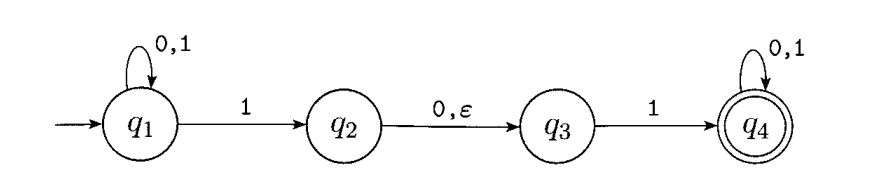
\includegraphics[width=0.5\linewidth]{images/ndautoma1}
\end{center}
La differenza fra un automa a stati finiti deterministico (\textit{DFA}, Deterministic Finite Automaton) e non deterministico  (\textit{NFA}, Nondeterministic Finite Automaton):
\begin{itemize}
	\item Ogni stato di un DFA ha esattamente una freccia uscente per ogni simbolo dell'alfabeto. Un NFA vìola questa regola.
	\item Un stato di un NFA può avere zero, una o più frecce uscenti per ogni simbolo dell'alfabeto (compreso $\varepsilon$).
\end{itemize}
\subsubsection{Come computa un NFA?}
Supponiamo di trovarci in un NFA con una stringa in input che ci ha condotti allo stato $q_1$ che ha più modi di procedere. Per esempio, diciamo che il prossimo simbolo di input è $1$. Dopo aver letto il simbolo la macchina si divide in copie multiple di se stessa e segue \textbf{tutte} le possibili vie in parallelo. Ogni copia della macchina prende una direzione e continua la computazione come prima, dividendosi a sua volta in più copie se necessario. Se il prossimo simbolo di input non compare in nessuna freccia uscente dallo stato corrente di ogni copia, quella copia cessa di esistere assieme al ramo della computazione a lei associato. Alla fine dell'input, se almeno una delle copie si trova in uno stato accettante, il NFA accetta la stringa di input. \\
Se viene incontrato uno stato con una freccia uscente con il simbolo $\varepsilon$, senza nemmeno leggere l'input la macchina se divide in copie multiple, una per ogni freccia uscente marcata da $\varepsilon$ e una copia rimane ferma sullo stato corrente. Successivamente la macchina procede in modo non deterministico come prima.
\begin{center}
	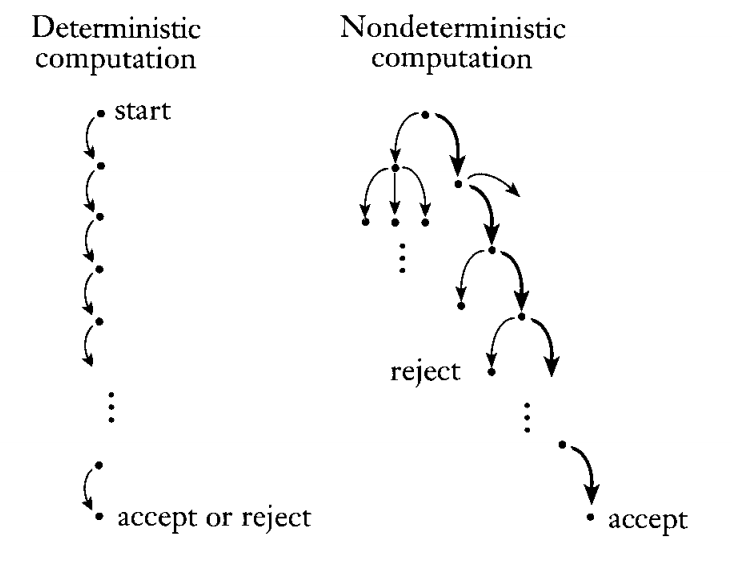
\includegraphics[width=0.5\linewidth]{images/nondeterministic}
\end{center}
\example di computazione non deterministica dell'automa visto sopra con l'input $010110$:
\begin{center}
	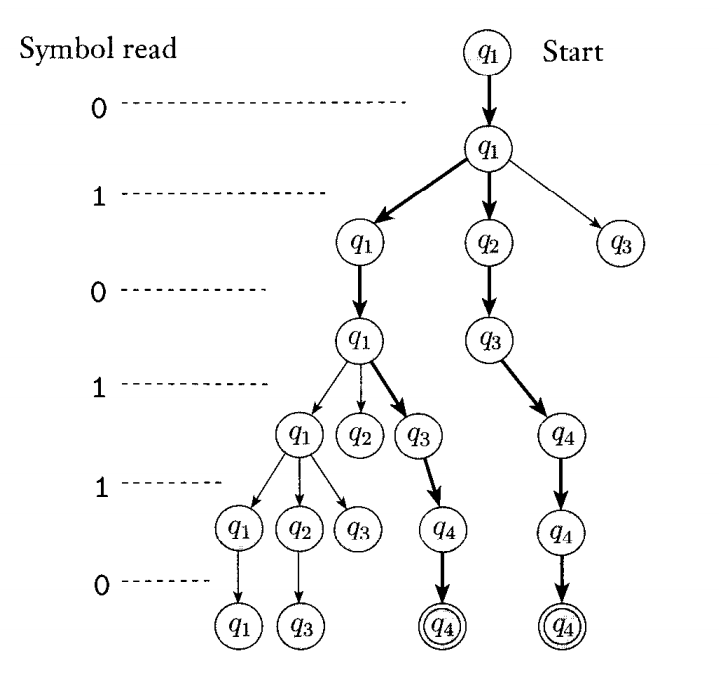
\includegraphics[width=0.7\linewidth]{images/branches}
\end{center}
\example: sia $A$ il linguaggio che consiste in tutte le stringhe in $\{0,1\}$ che contengono un $1$ nella terza posizione dalla fine (es. $000100$). Il seguente NFA a tre stati riconosce $A$:
\begin{center}
	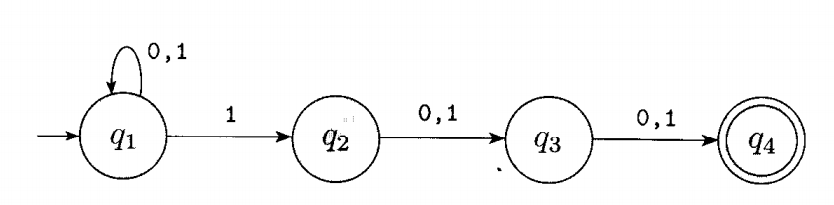
\includegraphics[width=0.5\linewidth]{images/nfa_1}
\end{center}
\pagebreak
\subsubsection{Definizione}
Una NFA è una quantupla $(Q,\;\Sigma,\;\delta,\;q_0,\;F)$ dove:
\begin{enumerate}
	\item $Q$ è un insieme finito di stati
	\item $\Sigma$ è un insieme finito di simboli detto alfabeto
	\item $\delta: Q\times (\Sigma \cup \{\varepsilon\}) \to \powerset{Q}$ 
	\item $q_0 \in Q$ è lo stato iniziale 
	\item $F \subseteq Q$ è un insieme degli stati finali 
\end{enumerate}
\example
\begin{center}
	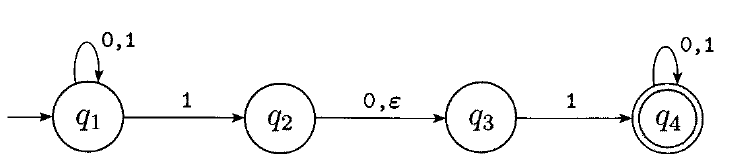
\includegraphics[width=0.7\linewidth]{images/nfa_2}
\end{center}
L'automa può essere rappresentato formalmente mediante la seguente sintassi:
\[
	A = (\{q_1,q_2,q_3,q_4\},\; \{0,1\},\; \delta,\; q_1,\; \{q_4\}) 
\]
dove $\delta$ è definita come:
\begin{table}[h!]
	\begin{tabular}{@{}llll}
			$\delta(q_1,0) = \{q_1\}$ & $\delta(q_2,0) = \{q_3\}$ & $\delta(q_3,0) = \varnothing$ & $\delta(q_4,0) = \{q_4\}$\\
			$\delta(q_1,1) = \{q_1,q_2\}$ & $\delta(q_2,1) = \varnothing$ & $\delta(q_3,1) = \{q_4\}$ & $\delta(q_4,1) = \{q_4\}$\\
			$\delta(q_1,\varepsilon) = \varnothing$ & $\delta(q_2,\varepsilon) = \{q_3\}$ & $\delta(q_3,\varepsilon) = \varnothing$ & $\delta(q_4,\varepsilon) = \varnothing$
	\end{tabular}
\end{table}
\subsubsection{Accettazione di una stringa}
Sia $N = (Q,\;\Sigma,\;\delta,\;q_0,\;F)$ un NFA. Diciamo che $N$ accetta una stringa $w$ nell alfabeto $\Sigma$ se e solo se $w$ può essere scritta nella forma $y_1,\dots,y_n$ dove $\forall i \in [1,n]:y_i \in \left( \Sigma \cup \{\varepsilon\} \right)$ ed esiste una sequenza di stati $R_0,\dots,R_n \in Q$ tali che:
\begin{itemize}
	\item $R_0$ è lo stato iniziale
	\item $R_m \in F$
	\item $\forall i \in [0,m-1]: R_{i+1} \in \delta(R_i,y_{i+1})$, ovvero che lo stato successivo ($R_{i+1}$) appartiene all'insieme degli stati ottenuti dalla funzione di transizione applicata allo stato corrente ($R_i$) e al prossimo carattere in input ($y_{i+1}$).
\end{itemize}
\subsubsection{Equivalenza tra NFA e DFA}
Dimostrare che ogni NFA ha un equivalente DFA.\\\\
Sia $N = (Q,\;\Sigma,\;\delta,\;q_0,\;F)$ un NFA che riconosce il linguaggio $A$, costruisco un DFA $M = (Q',\;\Sigma,\;\delta',\;q_0',\;F')$ che riconosce esattamente $A$. Assumiamo per semplicità che non vi siano $\varepsilon-$transizioni. Definiamo le componenti di $M$:
\begin{itemize}
	\item $Q' = \powerset{Q}$, insieme delle parti di $Q$
	\item $\delta'(R,a) = \bigcup\limits_{r\in R}\delta(r,a), \quad R \in Q', a \in \Sigma$
	\item $q_0'=\{q_0\}$
	\item $F' = \{R \in \powerset{Q} \;| \exists r \in R, r \in F\}$, ovvero esiste un insieme $R$ nell'insieme delle parti di $Q$ tale che $R$ contenga almeno uno stato accettante (finale) di $N$
\end{itemize}
Verifichiamo che le funzioni di transizione siano ben tipate:
\begin{enumerate}
	\item NFA: $\delta: Q \times \Sigma \to \powerset{Q}$
	\item DFA: $\delta': \underbracket{\powerset{Q}}_{Q'} \times \Sigma \to \underbracket{\powerset{Q}}_{Q'}$
\end{enumerate}
Generalizziamo ora il caso delle $\varepsilon$-transizioni definendo una funzione $E(R) = \{ q \;|\; q \in Q \}$ può essere raggiunto da uno stato in $R$ seguendo solamente $\varepsilon$-transizioni (anche zero). Riformulando i componenti visti sopra:
\begin{itemize}
	\item $\delta'(R,a) =  \bigcup\limits_{r\in R}E\left(\delta(r,a)\right)$
	\item $q_0 = E(\{q_0\})$
\end{itemize}
\subsubsection{Linguaggi regolari}
Andiamo a dimostrare che un linguaggio è regolare se e solo se esiste un NFA che lo riconosce. Dimostrazione:
\begin{itemize}[label={}]
	\item $\Rightarrow$ Se un linguaggio è regolare, per definizione esiste un DFA che lo riconosce. Ma un DFA è un caso speciale di un NFA, quindi la prima parte è dimostrata.
	\item $\Leftarrow$ Sia $A$ un linguaggio tale che $A$ è riconosciuto da un NFA. Per il teorema esiste un DFA che riconosce $A$, quindi $A$ è regolare.
\end{itemize}
\example di conversione di un NFA in un DFA \\\\
NFA:
\begin{center}
	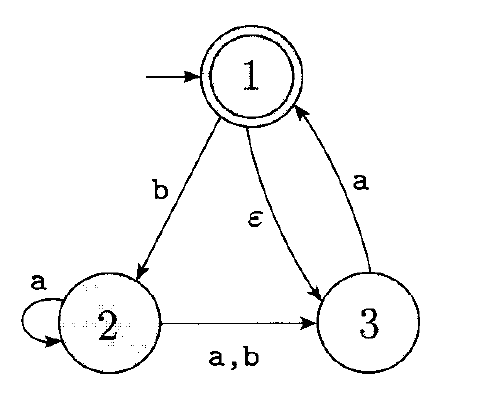
\includegraphics[width=0.3\linewidth]{images/nfa_3}
\end{center}
DFA:
\begin{center}
	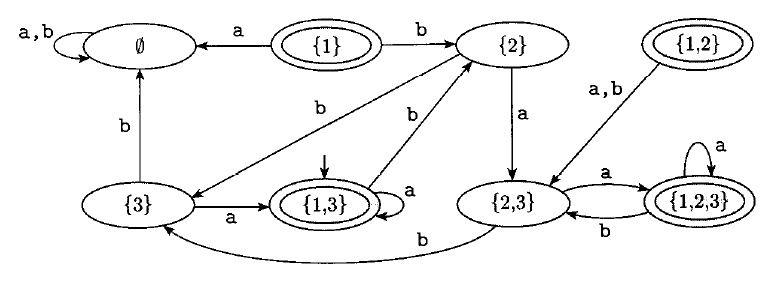
\includegraphics[width=0.7\linewidth]{images/nfa_4}
\end{center}
\paragraph{Chiusura rispetto all'unione}
La classe dei linguaggi regolari è chiusa rispetto all'unione. Dimostrazione: \\\\
Siano $A_1$ e $A_2$ due linguaggi regolari, allora esistono due NFA $N_1$ ed $N_2$ che li riconoscono. Costruisco da $N_1$ ed $N_2$ un NFA che riconosce $A_1\cup A_2$, da cui concludo che $A_1\cup A_2$ è regolare.
\begin{center}
	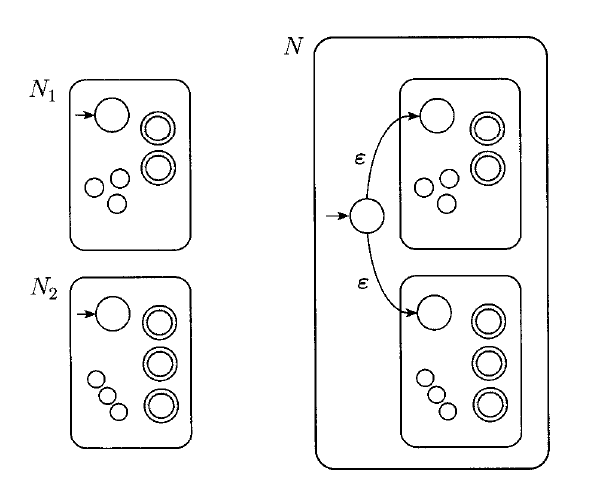
\includegraphics[width=0.7\linewidth]{images/nfa_union}
\end{center}
Definizione formale:
\[
	N_1 = (Q_1,\;\Sigma,\;\delta_1,\;q_1,\;F_1) \qquad N_2 = (Q_2,\;\Sigma,\;\delta_2,\;q_2,\;F_2)
\]
sia 
\[
	O = (Q,\;\Sigma,\;\delta,\;q_0,\;F)
\]
dove:
\begin{itemize}
	\item $Q = Q_1 \cup Q_2 \cup \{q_0\}$
	\item $F = F_1 \cup F_2$
	\item e la funzione di transizione è definita come
		\begin{align*}
		\delta(q,a) = 
		\begin{cases}
			\delta_1(q,a) & \text{se } q \in Q_1 \\
			\delta_2(q,a) & \text{se } q \in Q_2 \\
			\{q_1,q_2\} & \text{se } q=q_0 \land a = \varepsilon \\
			\varnothing & \text{se } q=q_0 \land a \neq \varepsilon 
		\end{cases}
		\end{align*}
\end{itemize}
\pagebreak
\paragraph{Chiusura rispetto alla concatenazione}
La classe dei linguaggi regolari è chiusa rispetto alla concatenazione. Dimostrazione: \\\\
Siano $A_1$ e $A_2$ due linguaggi regolari, allora esistono due NFA $N_1$ ed $N_2$ che li riconoscono.
\begin{center}
	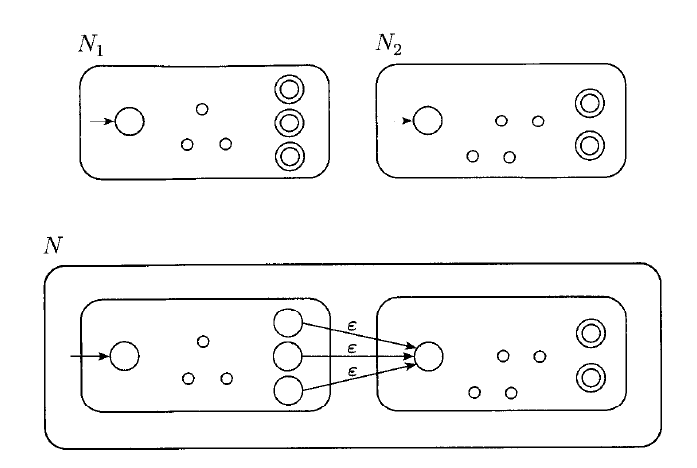
\includegraphics[width=0.7\linewidth]{images/nfa_concat}
\end{center}
In pratica salto dagli stati finali (non più) del primo automa allo stato iniziale del secondo automa. Definizione formale:
\[
	N_1 = (Q_1,\;\Sigma,\;\delta_1,\;q_1,\;F_1) \qquad N_2 = (Q_2,\;\Sigma,\;\delta_2,\;q_2,\;F_2)
\]
sia 
\[
	N = (Q,\;\Sigma,\;\delta,\;q_0,\;F)
\]
dove:
\begin{itemize}
	\item $Q = Q_1 \cup Q_2$
	\item $F = F_2$
	\item e la funzione di transizione è definita come
		\begin{align*}
			\delta(q,a) = 
			\begin{cases}
				\delta_1(q,a) & \text{se } q \in Q_1 \land q \notin F_1 \\
				\delta_1(q,a) & \text{se } q \in F_1 \land a \neq \varepsilon \\
				\delta_1(q,a) \cup \{q_2\} & \text{se } q \in F_1 \land a = \varepsilon\\
				\delta_2(q,a) & \text{se } q \in Q_2 
			\end{cases}
		\end{align*}
\end{itemize}



\end{document}
